% Options for packages loaded elsewhere
\PassOptionsToPackage{unicode}{hyperref}
\PassOptionsToPackage{hyphens}{url}
\PassOptionsToPackage{dvipsnames,svgnames,x11names}{xcolor}
%
\documentclass[
  letterpaper,
  DIV=11,
  numbers=noendperiod]{scrreprt}

\usepackage{amsmath,amssymb}
\usepackage{iftex}
\ifPDFTeX
  \usepackage[T1]{fontenc}
  \usepackage[utf8]{inputenc}
  \usepackage{textcomp} % provide euro and other symbols
\else % if luatex or xetex
  \usepackage{unicode-math}
  \defaultfontfeatures{Scale=MatchLowercase}
  \defaultfontfeatures[\rmfamily]{Ligatures=TeX,Scale=1}
\fi
\usepackage{lmodern}
\ifPDFTeX\else  
    % xetex/luatex font selection
\fi
% Use upquote if available, for straight quotes in verbatim environments
\IfFileExists{upquote.sty}{\usepackage{upquote}}{}
\IfFileExists{microtype.sty}{% use microtype if available
  \usepackage[]{microtype}
  \UseMicrotypeSet[protrusion]{basicmath} % disable protrusion for tt fonts
}{}
\makeatletter
\@ifundefined{KOMAClassName}{% if non-KOMA class
  \IfFileExists{parskip.sty}{%
    \usepackage{parskip}
  }{% else
    \setlength{\parindent}{0pt}
    \setlength{\parskip}{6pt plus 2pt minus 1pt}}
}{% if KOMA class
  \KOMAoptions{parskip=half}}
\makeatother
\usepackage{xcolor}
\setlength{\emergencystretch}{3em} % prevent overfull lines
\setcounter{secnumdepth}{5}
% Make \paragraph and \subparagraph free-standing
\ifx\paragraph\undefined\else
  \let\oldparagraph\paragraph
  \renewcommand{\paragraph}[1]{\oldparagraph{#1}\mbox{}}
\fi
\ifx\subparagraph\undefined\else
  \let\oldsubparagraph\subparagraph
  \renewcommand{\subparagraph}[1]{\oldsubparagraph{#1}\mbox{}}
\fi


\providecommand{\tightlist}{%
  \setlength{\itemsep}{0pt}\setlength{\parskip}{0pt}}\usepackage{longtable,booktabs,array}
\usepackage{calc} % for calculating minipage widths
% Correct order of tables after \paragraph or \subparagraph
\usepackage{etoolbox}
\makeatletter
\patchcmd\longtable{\par}{\if@noskipsec\mbox{}\fi\par}{}{}
\makeatother
% Allow footnotes in longtable head/foot
\IfFileExists{footnotehyper.sty}{\usepackage{footnotehyper}}{\usepackage{footnote}}
\makesavenoteenv{longtable}
\usepackage{graphicx}
\makeatletter
\def\maxwidth{\ifdim\Gin@nat@width>\linewidth\linewidth\else\Gin@nat@width\fi}
\def\maxheight{\ifdim\Gin@nat@height>\textheight\textheight\else\Gin@nat@height\fi}
\makeatother
% Scale images if necessary, so that they will not overflow the page
% margins by default, and it is still possible to overwrite the defaults
% using explicit options in \includegraphics[width, height, ...]{}
\setkeys{Gin}{width=\maxwidth,height=\maxheight,keepaspectratio}
% Set default figure placement to htbp
\makeatletter
\def\fps@figure{htbp}
\makeatother
% definitions for citeproc citations
\NewDocumentCommand\citeproctext{}{}
\NewDocumentCommand\citeproc{mm}{%
  \begingroup\def\citeproctext{#2}\cite{#1}\endgroup}
\makeatletter
 % allow citations to break across lines
 \let\@cite@ofmt\@firstofone
 % avoid brackets around text for \cite:
 \def\@biblabel#1{}
 \def\@cite#1#2{{#1\if@tempswa , #2\fi}}
\makeatother
\newlength{\cslhangindent}
\setlength{\cslhangindent}{1.5em}
\newlength{\csllabelwidth}
\setlength{\csllabelwidth}{3em}
\newenvironment{CSLReferences}[2] % #1 hanging-indent, #2 entry-spacing
 {\begin{list}{}{%
  \setlength{\itemindent}{0pt}
  \setlength{\leftmargin}{0pt}
  \setlength{\parsep}{0pt}
  % turn on hanging indent if param 1 is 1
  \ifodd #1
   \setlength{\leftmargin}{\cslhangindent}
   \setlength{\itemindent}{-1\cslhangindent}
  \fi
  % set entry spacing
  \setlength{\itemsep}{#2\baselineskip}}}
 {\end{list}}
\usepackage{calc}
\newcommand{\CSLBlock}[1]{\hfill\break\parbox[t]{\linewidth}{\strut\ignorespaces#1\strut}}
\newcommand{\CSLLeftMargin}[1]{\parbox[t]{\csllabelwidth}{\strut#1\strut}}
\newcommand{\CSLRightInline}[1]{\parbox[t]{\linewidth - \csllabelwidth}{\strut#1\strut}}
\newcommand{\CSLIndent}[1]{\hspace{\cslhangindent}#1}

\KOMAoption{captions}{tableheading}
\makeatletter
\@ifpackageloaded{bookmark}{}{\usepackage{bookmark}}
\makeatother
\makeatletter
\@ifpackageloaded{caption}{}{\usepackage{caption}}
\AtBeginDocument{%
\ifdefined\contentsname
  \renewcommand*\contentsname{Table of contents}
\else
  \newcommand\contentsname{Table of contents}
\fi
\ifdefined\listfigurename
  \renewcommand*\listfigurename{List of Figures}
\else
  \newcommand\listfigurename{List of Figures}
\fi
\ifdefined\listtablename
  \renewcommand*\listtablename{List of Tables}
\else
  \newcommand\listtablename{List of Tables}
\fi
\ifdefined\figurename
  \renewcommand*\figurename{Figure}
\else
  \newcommand\figurename{Figure}
\fi
\ifdefined\tablename
  \renewcommand*\tablename{Table}
\else
  \newcommand\tablename{Table}
\fi
}
\@ifpackageloaded{float}{}{\usepackage{float}}
\floatstyle{ruled}
\@ifundefined{c@chapter}{\newfloat{codelisting}{h}{lop}}{\newfloat{codelisting}{h}{lop}[chapter]}
\floatname{codelisting}{Listing}
\newcommand*\listoflistings{\listof{codelisting}{List of Listings}}
\makeatother
\makeatletter
\makeatother
\makeatletter
\@ifpackageloaded{caption}{}{\usepackage{caption}}
\@ifpackageloaded{subcaption}{}{\usepackage{subcaption}}
\makeatother
\ifLuaTeX
  \usepackage{selnolig}  % disable illegal ligatures
\fi
\usepackage{bookmark}

\IfFileExists{xurl.sty}{\usepackage{xurl}}{} % add URL line breaks if available
\urlstyle{same} % disable monospaced font for URLs
\hypersetup{
  pdftitle={Applied Data Science},
  pdfauthor={Haseeb Mahmud},
  colorlinks=true,
  linkcolor={blue},
  filecolor={Maroon},
  citecolor={Blue},
  urlcolor={Blue},
  pdfcreator={LaTeX via pandoc}}

\title{Applied Data Science}
\author{Haseeb Mahmud}
\date{2025-09-27}

\begin{document}
\maketitle

\renewcommand*\contentsname{Table of contents}
{
\hypersetup{linkcolor=}
\setcounter{tocdepth}{2}
\tableofcontents
}
\bookmarksetup{startatroot}

\chapter*{Welcome note}\label{welcome-note}
\addcontentsline{toc}{chapter}{Welcome note}

\markboth{Welcome note}{Welcome note}

Dear students,

In this part of this course, we are going to cover the practical part of
the course, which is the application of different

\begin{enumerate}
\def\labelenumi{\arabic{enumi}.}
\tightlist
\item
\end{enumerate}

\bookmarksetup{startatroot}

\chapter{What is research}\label{what-is-research}

When listening to the radio, watching the television or reading a daily
newspaper it is difficult to avoid the term `research'. The results of
`research' are all around us. A debate about the findings of a recent
poll of people's opinions inevitably includes a discussion of
`research', normally referring to the way in which the data were
collected. Politicians often justify their policy decisions on the basis
of `research'. Newspapers report the findings of research companies'
surveys. Documentary programs tell us about `research findings', and
advertisers may highlight the `results of research' to encourage you to
buy a particular product or brand. However, we believe that what these
examples really emphasizes is the wide range of meanings given to the
term `research' in everyday speech.

Walliman (2005) argues that many of these everyday uses of the term
`research' are not research in the true meaning of the word. As part of
this, he highlights ways in which the term is used wrongly:

\begin{itemize}
\tightlist
\item
  just collecting facts or information with no clear purpose;
\item
  reassembling and reordering facts or information without
  interpretation;
\item
  as a term to get your product or idea noticed and respected.
\end{itemize}

The first of these highlights the fact that, although research often
involves the collection of information, it is more than just reading a
few books or articles, talking to a few people or asking people
questions. While collecting data may be part of the research process, if
it is not undertaken in a systematic way, on its own and, in particular,
with a clear purpose, it will not be seen as research. The second of
these is commonplace in many reports. Data are collected, perhaps from a
variety of different sources, and then assembled in a single document
with the sources of these data listed. However, there is no
interpretation of the data collected. Again, while the assembly of data
from a variety of sources may be part of the process of research,
without interpretation it is not research. Finally, the term `research'
can be used to get an idea or product noticed by people and to suggest
that people should have confidence in it. In such instances, when you
ask for details of the research process, these are either unclear or not
forthcoming. (See Saunders, Lewis, and Thornhill 2019)

In short, research is a diligent search, studious inquiry or
investigation or experimentation aimed at the discovery of new facts and
findings; or broadly, it may relate to any subject of inquiry with
regard to collection of information, interpretation of facts, revision
of existing theories or laws in the light of new facts or practical
ideas. (See Adams, Khan, and Raeside 2014)

Based upon this brief discussion we can already see that research has a
number of characteristics:

\begin{itemize}
\tightlist
\item
  Data are collected systematically.
\item
  Data are interpreted systematically.
\item
  There is a clear purpose: to find things out.
\end{itemize}

We can therefore define research as something that people undertake in
order to find out things in a systematic way, thereby increasing their
knowledge. Two phrases are important in this definition: `systematic
way' and `to find out things'. `Systematic' suggests that research is
based on logical relationships and not just beliefs (Ghauri and Grønhaug
(2002)). As part of this, your research will involve an explanation of
the methods used to collect the data, will argue why the results
obtained are meaningful, and will explain any limitations that are
associated with them. `To find out things' suggests there are a
multiplicity of possible purposes for your research. These may include
describing, explaining, understanding, criticizing and analyzing (Ghauri
and Grønhaug (2002)). However, it also suggests that you have a clear
purpose or set of `things' that you want to find out, such as the answer
to a question or number of questions (See Saunders, Lewis, and Thornhill
2019).

\section{Research method vs.~research
methodology}\label{research-method-vs.-research-methodology}

A research method is a way of conducting and implementing research. The
term `methods' refers to specific activities (e.g.~designing
questionnaire, conducting interviews, focus groups, observation etc.).
On the other hand, research methodology is the science and philosophy
behind all research. It is more about our attitude to and our
understanding of research and the strategy or approach you choose to
answer research questions.

\section{Why is research conducted}\label{why-is-research-conducted}

Research is conducted for a number of reasons, which in turn depend on
the objectives of any particular `research problem'. It may be to find
out something we do not already know or to enhance our understanding of
phenomena that we already know something about. In the business arena,
however, research tends to be undertaken in order to achieve one or more
of the following objectives (Adams, Khan, and Raeside 2014):

\begin{itemize}
\tightlist
\item
  To gain a competitive advantage
\item
  To test new products and services
\item
  To solve a management/organisational problem
\item
  To provide information, which may help to avoid future business
  problems
\item
  To forecast future sales
\item
  To better understand shifts in consumer attitudes and tastes
\item
  To enhance profitability
\item
  To reduce operational costs
\item
  To enable the management to priorities strategic options for the
  future etc.
\end{itemize}

\section{Approaches to business and social
research}\label{approaches-to-business-and-social-research}

Researchers usually handle numerous problems and apply research methods
to obtain the best guess answers to their questions. They may use a
single study or a combination of two designs. The investigator has to
decide about the types and combinations of research forms that best
serve the goals of the study. Broadly speaking, there are two main
domains of research frequently observed in the literature, which are
Quantitative research and Qualitative research. It is possible to
combine quantitative and qualitative together to answer a single
research question. Those approaches are known as mixed method research
works. The diverse practices and uses of today's research practices are
listed in the following paragraphs.

\begin{itemize}
\tightlist
\item
  Quantitative research
\item
  Qualitative research
\item
  Pure theoretical research
\item
  Applied research
\item
  Longitudinal studies
\item
  Theory vs.~empirical study
\end{itemize}

\section{The research process}\label{the-research-process}

\begin{figure}

\centering{

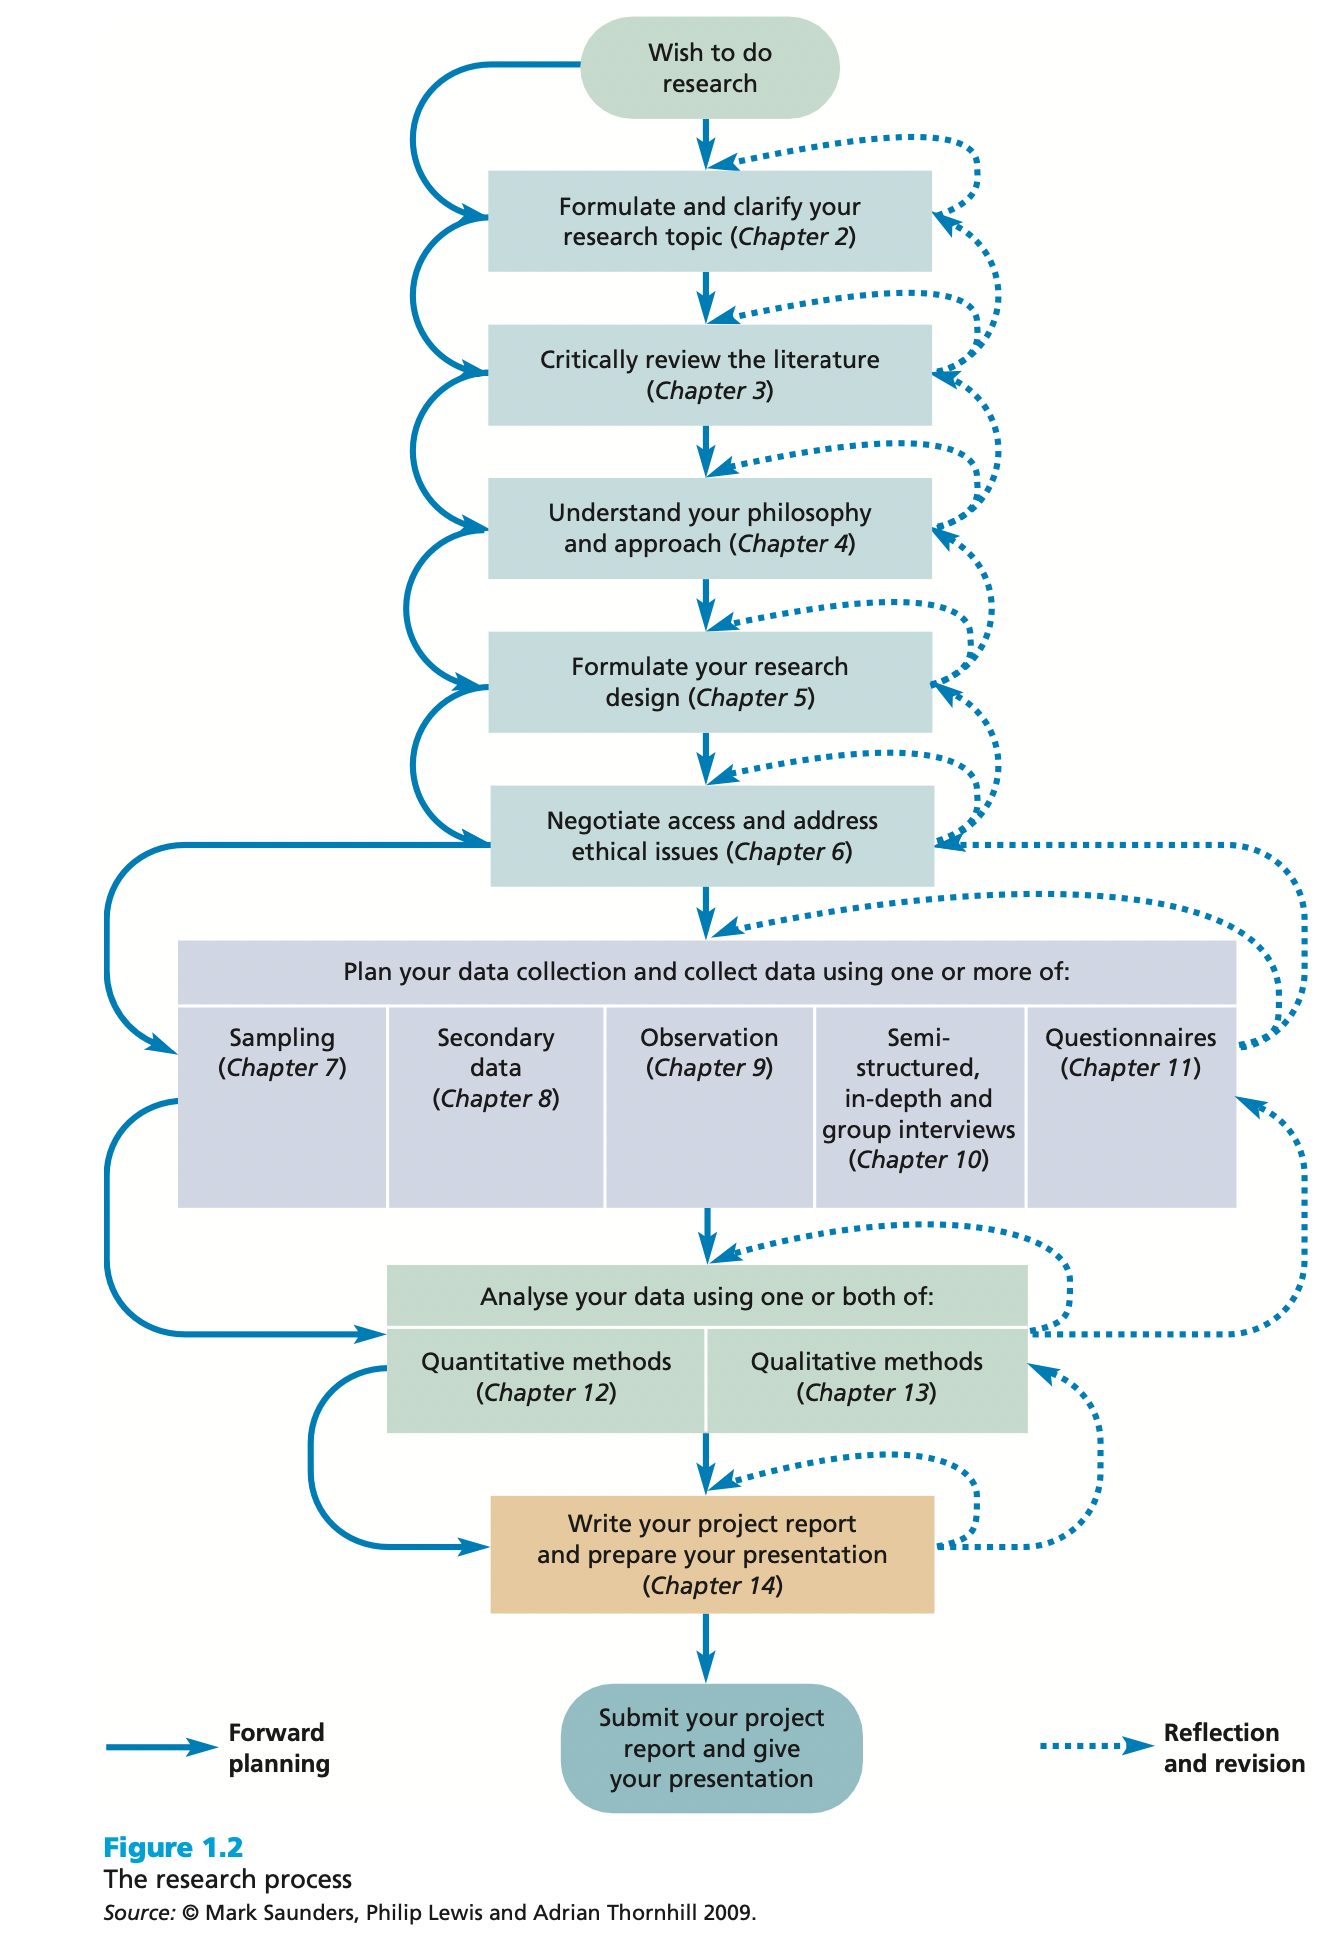
\includegraphics{images/SCR-20221004-gg4.png}

}

\caption{\label{fig-res_process}The Research process (Saunders, Lewis,
and Thornhill (2019))}

\end{figure}%

\section{The hallmarks of scientific
research}\label{the-hallmarks-of-scientific-research}

The hallmarks or main distinguishing characteristics of scientific
research may be listed as follows (Bougie and Sekaran (2020)):

\begin{itemize}
\tightlist
\item
  Purposiveness
\item
  Rigor
\item
  Testability
\item
  Replicability
\item
  Precision and confidence
\item
  Objectivity
\item
  Generalizability
\item
  Parsimony
\end{itemize}

\bookmarksetup{startatroot}

\chapter*{References}\label{references}
\addcontentsline{toc}{chapter}{References}

\markboth{References}{References}

\phantomsection\label{refs}
\begin{CSLReferences}{1}{0}
\bibitem[\citeproctext]{ref-adams_research_2014}
Adams, John, Hafiz T. A. Khan, and R. Raeside. 2014. \emph{Research
Methods for Business and Social Science Students}. Second edition. Los
Angeles: SAGE.

\bibitem[\citeproctext]{ref-bougie_research_2020}
Bougie, Roger, and Uma Sekaran. 2020. \emph{Research Methods for
Business: A Skill-Building Approach}. Eight edition. Hoboken, NJ: Wiley.

\bibitem[\citeproctext]{ref-ghauri_research_2002}
Ghauri, Pervez N., and Kjell Grønhaug. 2002. \emph{Research Methods in
Business Studies: A Practical Guide}. 2nd ed. Harlow, England ; New
York: Financial Times Prentice Hall.

\bibitem[\citeproctext]{ref-saunders_research_2019}
Saunders, M. N. K., Philip Lewis, and Adrian Thornhill. 2019.
\emph{Research Methods for Business Students}. Eighth Edition. New York:
Pearson.

\bibitem[\citeproctext]{ref-walliman_your_2005}
Walliman, Nicholas. 2005. \emph{Your Research Project: A Step-by-Step
Guide for the First-Time Researcher}. 2nd ed. London ; Thousand Oaks,
Calif: Sage Publications.

\end{CSLReferences}



\end{document}
